\documentclass[12pt,a4paper]{article}
%\usepackage{epsf,epic,eepic,eepicemu}
%\documentstyle[epsf,epic,eepic,eepicemu]{article}

\usepackage[pdftex]{graphicx}
\usepackage[utf8]{inputenc} %kodovani znaku v textovem souboru
%\usepackage[T1]{fontenc} %kodovani znaku na vystupu
\usepackage[czech]{babel} %prizpusobeni jazyku, napr. deleni slov
%\usepackage{a4wide}

\begin{document}
\title{Semestrální projekt MI-PPR.2 2014/2015\\
Paralelní algoritmus pro řešení problému \\
\vspace{10px}}
\author{Karel Fiala \\ Michal Kučera \\
\vspace{10px} \\
\small České vysoké učení technické v Praze\\
\small Fakulta informačních technologií\\
\small Thákurova 9, 160 00 Praha 6\\
\small Česká republika \\
\vspace{10px} \\
}
\date{\today}
\maketitle

%\oddsidemargin=-5mm \evensidemargin=-5mm \marginparwidth=.08in
%\marginparsep=.01in \marginparpush=5pt \topmargin=-15mm
%\headheight=12pt \headsep=25pt \footheight=12pt \footskip=30pt
%\textheight=25cm \textwidth=17cm \columnsep=2mm \columnseprule=1pt
%\parindent=15pt\parskip=2pt

%Zpráva má obsahovat minimálně následující body:

%Definici problému
%Popis sekvenčního algoritmu a jeho implementace
%Popis paralelního algoritmu a jeho implementace, včetně odůvodnění volby algoritmu pro hledání dárce a metody dělení zásobníku
%Tabulkově a případně graficky zpracované naměřené hodnoty časové složitosti měřených instancí běhu programu s popisem instancí dat
%Analýza a hodnocení vlastností paralelního programu, zvláště jeho efektivnosti a škálovatelnosti, vzniku superlineárního zrychlování a srovnání komunikační režie stejných instancí nad Ethernetem a Infinibandem.
%Závěr
%Literatura

\clearpage
\tableofcontents
\clearpage

\section{Definice problému a popis sekvenčního algoritmu}

%Popište problém, který váš program řeší. Jako výchozí použijte text
%zadání, který rozšiřte o přesné vymezení všech odchylek, které jste
%vůči zadání během implementace provedli (např.  úpravy heuristické
%funkce, organizace zásobníku, apod.). Zmiňte i případně i takové
%prvky algoritmu, které v zadání nebyly specifikovány, ale které se
%ukázaly jako důležité.  Dále popište vstupy a výstupy algoritmu
%(formát vstupních a výstupních dat). Uveďte tabulku nameřených časů
%sekvenčního algoritmu pro různě velká data.

\subsection{Úloha PEK: Permutace číselných koleček}

\subsubsection{Vstupní data}

$ n = $ délka rovnostranného trojúhelníka, $ n >= 5 $ \\
$ q = $ přirozené číslo, $n^{2} > q $ \\
$ X_{0} = $ počáteční konfigurace zkonstruovaná zpětným provedením $ q $ náhodných tahu z cílové konfigurace. Platí $ q>=d(X_{0}) $. \\
\begin{verbatim}
./balls.out <n> <q> <data file>
\end{verbatim}

\subsubsection{Pravidla a cíl hry}

Herní deska má tvar rovnostranného trojúhelníka o délce strany n, kde v i-tem řádku je i políček, ležících na průsečících úseček, rovnoběžných se stranami trojúhelníka. V těchto políčkách jsou podle určité permutace rozmístěna kolečka s čísly $ 1, \dots ,M-1 $, kde $ M=n(n+1)/2 $. Jedno políčko zůstává volné, viz příklad na obrázku \ref{pek}.

\begin{figure}[ht]
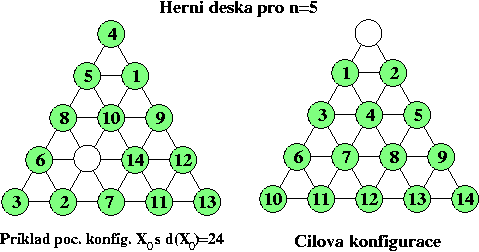
\includegraphics[width=\textwidth]{pek.png}
\caption{Hrací plocha}
\label{pek}
\end{figure}

Tomuto rozmístění koleček budeme říkat počáteční konfigurace $ X_{0} $. Jeden tah je přesun kolečka na sousední volné políčko ve směru některé úsečky. Cílem hry je použitím minimálního počtu tahů převést počáteční konfiguraci $ X_{0} $ do cílové konfigurace $ C $, ve které jsou kolečka seřazena vzestupně po řádcích tak, že políčko na horním vrcholu trojúhelníkové desky je volné, viz obrázek vpravo. Úloha má vždy řešení.

\subsubsection{Definice}

Je-li $ X $ konfigurace rozmístění všech koleček na herní desce, pak $ t_{X} $ je počet doposud provedených tahů, kterými jsme převedli počáteční konfiguraci $ X_{0} $ do konfigurace $ X $.

$ d_{X} $ je spodní mez počtu tahů, kterými se lze dostat z konfigurace $ X $ do cílové konfigurace $ C $. Tato spodní mez je rovna součtu vzdáleností koleček od jejich cílových políček. Vzdálenost 2 políček v této síti se počítá takto: Jsou-li obě políčka na úsečce rovnoběžné se stranou trojúhelníka, pak je vzdálenost rovna jejich lineární vzdálenosti po této úsečce. V opačném případě tvoří políčka vrcholy kosodélníka a vzdálenost se rovná součtu délek jeho dvou stran. Spodní mez počtu tahů nejlepšího možného řešení je tedy $ d_{X_{0}} $.

Generování počátečního stavu: $ X_{0} $ vygenerujeme nejprve $ q $ náhodně provedenými zpětnými tahy z cílové konfigurace $ C $.

\subsubsection{Výstup algoritmu}

Výpis nejkratší posloupnosti tahů vedoucí z počáteční konfigurace do cílové konfigurace.\\
\\
\textbf{Odchylka od zadání:} Výpis nejmenšího počtu tahů vedoucí z počáteční konfigurace do cílové konfigurace.

\subsubsection{Sekvenční algoritmus}

Sekvenční algoritmus je typu BB-DFS s neomezenou hloubkou stromu konfiguraci. Přípustný stav je cesta z počáteční do cílové konfigurace $ C $. Cena, která se minimalizuje, je počet tahů takové cesty.\\
\\
Horní mez počtu tahů je $ q $.
\\
Dolní mez je $ d_{X_{0}} $.

\subsubsection{Paralelní algoritmus}

Paralelní algoritmus je typu L-PBB-DFS-D.\\
\\
\textbf{Odchylka od zadání:} Implementovali jsme algoritmus typu G-PBB-DFS-D. Důvodem bylo zrychlení hledání řešení, pomocí dynamického zkracování prohledávaného prostoru.



\section{Popis paralelního algoritmu a jeho implementace v MPI}

\subsection{Odlišnost od sekvenčního algoritmu}
Paralelní algoritmus se výpočetně neliší od sekvenčního algoritmu. O celou komunikaci v MPI se stará jedna funkce, která je volána ze \uv{sekvenčního algoritmu} v případě, že
\begin{itemize}
\item nemá proces práci (zásobník je prázdný)
\item proces nalezl nové řešení 
\item proces vykonal $ XYZ $ kroků
\end{itemize}
\medskip

\subsection{Směr komunikace}
Celá komunikace probíhá jedním směrem v kruhu. Procesy žádají o prácí proces číslo $ MyRank - 1 $ a naopak práci posílají procesu s číslem $ MyRank + 1 $.\\

\subsection{Práce se zásobníkem}
Zásobník se spravedlivě půlí a posílá se vždy spodní část zásobníku. Tím nedochází k situace, že by nejlehčí konfigurace byla zpracována až jako poslední. Díky rozdělení výpočetně naročnějších konfigurací ze dna zásobníku také klesá potřeba komunikace a přerozdělování práce, což se pozitivně odráží na lineárním zrychlení paralelního algoritmu.\\

\subsection{Ukončení výpočtu}
Ukončení výpočtu je realizováno pomocí $ token $ ve formě čítače. Každý proces, který od doby inicializace žádosti o ukončení dostane práci, najde výsledek nebo \uv{uslyší} o novém výsledku, tento čítač resetuje na počáteční hodnotu a nedojde tak k předčasnému ukončení výpočtu. O inicializaci žádosti o ukončení a případně o ukončení výpočtu vždy rozhoduje proces s číslem $0$.\\

\medskip

\subsection{Parametry algoritmu}
Zapne dynamického zkracování prohledávaného prostoru na základě již známých výsledků. Tento parametr však \uv{maskuje} linearitu zrychlení a proto byl pro potřeby měření vypnut.
\begin{verbatim}
#define SMART_SEARCH 1
\end{verbatim}

\bigskip

Parametr, který určuje frekvenci komunikace. Jedná se o počet konfigurací, které budou vyřešeny před zavolám komunikačního okénka.
\begin{verbatim}
#define COMWIN_REQ_STEPS 100
\end{verbatim}

\medskip

\subsection{Spouštění}
Program spouštíme
\begin{verbatim}
./balls.out <n> <q> <data file>
\end{verbatim}

\section{Naměřené výsledky a vyhodnocení}

\subsection{Ethernet vs. Infiniband}
Na námi navrženém algoritmu se rozdíl mezi komunikační sítí \textbf{Infiniband} ($41,4s$) a \textbf{Ethernet} ($39,8s$) neprojevil. Všechny rozdíly měření byly menší než odchylka měření. Vysvětlujeme si to tím, že náš algoritmus přenáší pouze nezbytně nutné a výpočetně výhodné informace a také heterogenní prostředí clusteru STAR s sebou přináší velkou odchylku měření (až $ 8\% $).\\

\subsection{Konfigurace měření}

\subsubsection{Spouštění}
Všechny uvedené hodnoty byly naměřeny s komunikační sítí \textbf{Infiniband} a spuštěny pomocí:\\
\begin{verbatim}
qrun.sh 24c #CPU long <skript s konfigurací>
\end{verbatim}


\subsubsection{Konfigurace dimenze a horní mez}
\begin{verbatim}
./balls <dimenze> <horní mez> <data>
./balls n 			q 			data_n

./balls 4 19 triangle4
./balls 5 17 triangle5
./balls 6 15 triangle6
\end{verbatim}



\subsubsection{Datové soubory}
$ -1 $ reprezentuje prázdné políčko.

\paragraph{Soubor: triangle4}
\begin{verbatim}
1
3 2
8 4 5
6 7 -1 9
\end{verbatim}

\paragraph{Soubor: triangle5}
\begin{verbatim}
4
5 1
8 3 9
6 -1 2 7
10 11 12 13 14
\end{verbatim}

\paragraph{Soubor: triangle6}
\begin{verbatim}
4
5 1
2 3 7
6 -1 8 9
10 11 12 13 14
15 16 17 18 19 20
\end{verbatim}

\medskip


\subsection{Tabulka s výsledky}
\begin{center}
\begin{tabular}{ | c || c | c | c | }
\hline
\#CPU    &   triangle4		&	triangle5	&	triangle6	\\
\hline
\hline
1    &   478.645257		&	868.954290	&	287.384048		\\ \hline
2    &   294.697964		&	459.874666	&	177.874139		\\ \hline
4    &   126.608475		&	259.122906	&	97.633753		\\	 \hline
8    &   86.888339		&	146.344138	&	44.997678		\\	 \hline
16   &   52.924784		&	100.802686	&	32.854664		\\	 \hline
24   &   33.590004		&	60.888389	&	18.830592		\\ \hline
32   &   27.893136		&	42.098020	&	14.369734		\\ \hline
\end{tabular}
\end{center}

\clearpage
\subsection{Grafy}

Na grafech lineárního zrychlení $ S(n,p) $ je zobrazen naměřený čas, přibližná odchylka měření a průběh lineárního zrychlení, který vychází z naměřené hodnoty sekvenčního řešení.

\begin{figure}[h]
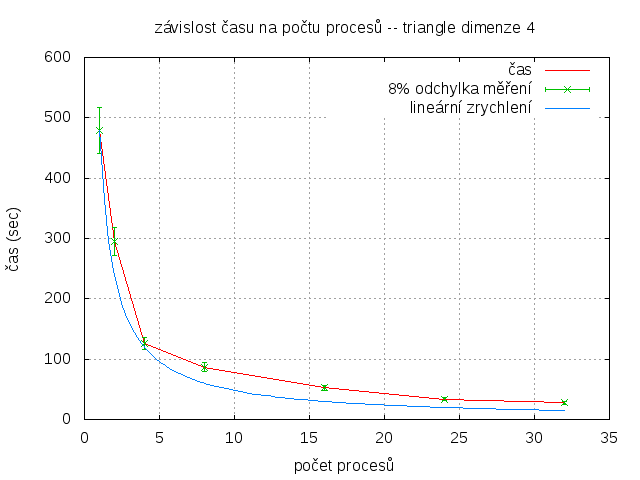
\includegraphics[width=\textwidth]{data4.png}
\caption{Měření pro trojúhelník dimenze 4}
\label{data4}
\end{figure}

\begin{figure}[h]
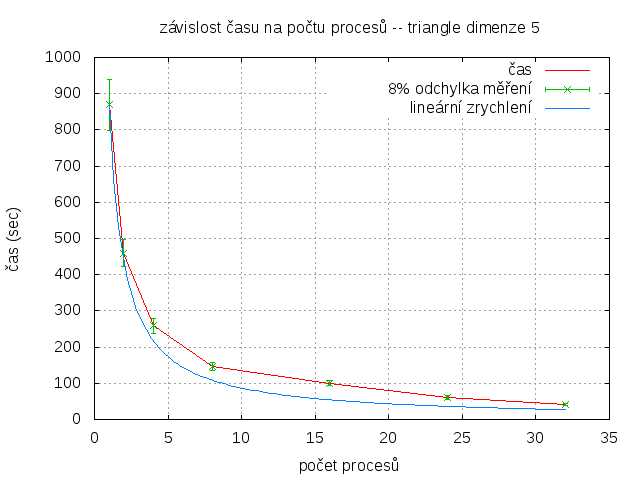
\includegraphics[width=\textwidth]{data5.png}
\caption{Měření pro trojúhelník dimenze 5}
\label{data5}
\end{figure}

\begin{figure}[h]
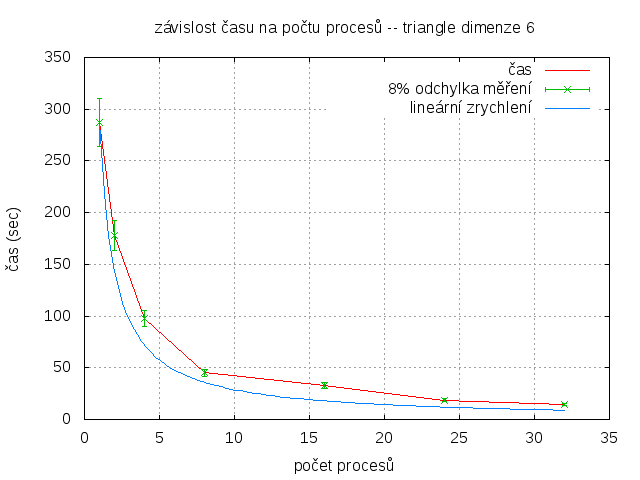
\includegraphics[width=\textwidth]{data6.png}
\caption{Měření pro trojúhelník dimenze 6}
\label{data6}
\end{figure}

\clearpage

\subsection{Vyhodnocení}

Zrychlení je lineární. \\

Díky prohledávání stavového prostoru do hloubky je algoritmus paměťově nenáročný a nevzniká tak superlineární zrychlení.


\section{Závěr}

Zkušenost s MPI je velkým přínosem, stejně tak i oživení programování v $ C/C++ $.\\

Překvapilo nás relativně snadné použití knihovny MPI.\\


\end{document}
